\documentclass[xcolor=pdftex,dvipsnames,table,mathserif,aspectratio=169]{beamer}
\usetheme{metropolis}
%\usetheme{Darmstadt}
%\usepackage{times}
%\usefonttheme{structurebold}

\usepackage[english]{babel}
%\usepackage[table]{xcolor}
\usepackage{pgf,pgfarrows,pgfnodes,pgfautomata,pgfheaps}
\usepackage{amsmath,amssymb,setspace,outline}
\usepackage[latin1]{inputenc}
\usepackage[T1]{fontenc}
\usepackage{relsize}
\DeclareMathSizes{10}{10}{6}{6} 


\title [Single-agent dynamic optimization models]{Numerical Dynamic Programming}
\author{Chris Conlon  }
\institute{Grad IO}
\date{\today }
\setbeamerfont{equation}{size=\tiny}
\begin{document}

\begin{frame}
\titlepage
\end{frame}

\begin{frame}{Reading}
\begin{itemize}
\item Rust 1994 "Numerical Dynamic Programming in Economics" (Handbook Chapter)
\item SLP Chapter 9: Stochastic Dynamic Programming (Theory)
\item Judd Chapter 6: Approximation Methods
\item Judd Chapter 7: Numerical Integration
\item Judd Chapter 11: Projection Methods
\item Judd Chapter 12: Numerical Dynamic Progrmamming
\end{itemize}
\end{frame}


\begin{frame}{MDP Definition}
\begin{itemize}
\item A time index $t \in\{0,1,2,\ldots,T\}$, with $T \leq \infty$
\item A state space $S$
\item A decision space $A$
\item A family of constraint sets $A_t(s_t) \subseteq A$
\item A family of transition probabilities $p_{t+1}(\cdot | s_t,a_t)$, and $\mathfrak{B}(S) \rightarrow [0,1]$\footnote{$\sigma$ algebra of measurable subsets of $s$...blah blah}
\item A family of discount $\beta_t(s_t,a_t ) \geq 0$ and a single period utility function $u_t(s_t,a_t)$ such that the utility functional $U$ has the additively separable decomposition
\end{itemize}
\begin{eqnarray*}
U(s,a) = &\sum_{t=0}^T \left [ \prod_{j=0}^{t-1} \beta_j (s_j,a) \right] u_t(s_t,a_t) \\
\alpha(s) =&\arg \max_{\delta=(a_0,\ldots,a_T)} E_{a} U(s,a)
\end{eqnarray*}
\end{frame}


\begin{frame}{Characterizations of MDPs}
\begin{description}
\item[Finite Horizon] have $T < \infty$. Can compute $a^*$ by backward induction starting in the terminal period $T$.
\item[Infinite Horizon] $T=\infty$ use a recursive definition of the value function
\item[Discrete State Space] solve problems up to machine precision. (Good for estimation).  How realistic?
\item[Infinite State Space] most of economics, numerical approximation $\rightarrow$  errors and interactions of approximation errors.
\item [Discrete Decision Process] $D$ takes on a discrete set of values $\{a_1,\ldots,a_J\}$
\item[Continuous Decision Process (CDP)] These are tricky -- there are results about how well they can be approximated by DDPs and they are not overwhelmingly positive. (See Rust 1994).
\end{description}
\end{frame}

\begin{frame}{Examples of MDPs}
\begin{itemize}
\item Entry/Exit decisions of firms
\item R\&D Investment
\item Replacement of Durables
\item Consumer Search
\item Advertising?
\end{itemize}
\end{frame}

\begin{frame}{Bellman's Equation}
It is helpful to consider $V(s)$ as the solution to the MDP.  
\begin{eqnarray*}
V(s) = \max_{a \in A(s)} [ u(s,a) + \beta \int V(s') p(ds' | s,a)]
\end{eqnarray*}
This is a \alert{functional equation} and $V$ represents a \alert{fixed point} to the functional equation.\\
\vspace{0.5cm}
We are interested in existence/uniqueness of a solution to Bellman's Equation:
\begin{enumerate}
\item $A$ and $S$ are complete metric spaces
\item $u(s,a)$ is jointly continuous and bounded in $(s,a)$
\item $s \rightarrow A(s)$ is a continuous correspondence
\end{enumerate}
\end{frame}

\begin{frame}{Bellman Operator}
Helpful to rewrite Bellmans equation as an operator $V = \Gamma(V)$ where $\Gamma: \mathfrak{B}(S) \rightarrow \mathfrak{B}(S)$ (Measurable, bounded) \\
\vspace{0.5cm}
The Bellman operator has the contraction mapping property which guarantees a unique fixed point point in $B$.
\begin{eqnarray*}
\| \Gamma(V) - \Gamma(W) \| \leq \beta \| V-W \| \quad \forall V,W \in B
\end{eqnarray*}
\begin{block}{Blackwell's Theorem}
\textit{The stationary, Markovian, infinite horizon policy given by $\alpha(s)$ (the solution to Bellman's equation)  constitutes an optimal decision rule for the infinite horizon MDP.}
\end{block}
\end{frame}

\begin{frame}{Simple Case}
Start by thinking about \textit{Discrete Decision Problems} with a \textit{Discrete State Space}.  We can generalize to harder problems later.
\end{frame}

\begin{frame}{Solution Method: Finite Horizon Problems}
\begin{itemize}
\item The optimal decision depends only on the state $a_t = a(s_t)$ not the whole history because $p$ is markovian flow utilities are additively separable.
\item See this by thinking about choosing a unique $a_T(s_t)$ in the ultimate period (unless there are ties) hence randomization can only make the agent worse off.
\item All prior $d_t$'s are now deterministic functions of $s_t$ and so on
\item At time $t=0$ the value function $V_0^T(s_0)$ represents the conditional expectation of utility over all future periods> it follows that $V_0^T(s) = \max_{a} E_{a}\{ U(\tilde{s},\tilde{d}) | s_0 = s\}$.
\end{itemize}
\end{frame}

\begin{frame}{Solution Method: Value Function Iteration}
\begin{itemize}
\item Well known, basic algorithm of dynamic programming
\item Based on our backward induction method of solving finite-horizon problems.
\item We have tight convergence properties and bounds on errors
\item Well suited for parallelization
\item It is linearly convergent (slow depends on modulus of contraction mapping).
\end{itemize}
\end{frame}

\begin{frame}{Value Function Iteration: Finite Horizon}
Begin with the Bellman operator:
\begin{eqnarray*}
\Gamma(V^t)(s) = \max_{a \in A(s)} \left[ u(s,a) + \beta \int V^{t+1}(s')p(ds' | s,a) \right]
\end{eqnarray*}
Specify $V^T$ and apply the Bellman operator:
\begin{eqnarray*}
\Gamma(V^{T-1})(s) = \max_{a \in A(s)} \left[ u(s,a) + \beta \int V^{T}(s')p(ds' | s,a) \right]
\end{eqnarray*}
Iterate to first period:
\begin{eqnarray*}
\Gamma(V^1)(s) = \max_{a \in A(s)} \left[ u(s,a) + \beta \int V^{2}(s')p(ds' | s,a) \right]
\end{eqnarray*}
\end{frame}

\begin{frame}{Value Function Iteration: Infinite Horizon}
Begin with the Bellman operator:
\begin{eqnarray*}
\Gamma(V^k)(s) = \max_{a \in A(s)} \left[ u(s,a) + \beta \int V^{k+1}(s')p(ds' | s,a) \right]
\end{eqnarray*}
Specify $V^0$ and apply the Bellman operator:
\begin{eqnarray*}
V^{1}(s) = \max_{a \in A(s)} \left[ u(s,a) + \beta \int V^{0}(s')p(ds' | s,a) \right]
\end{eqnarray*}
Iterate until convergence  $ \sup_s \| \Gamma(V^k)(s) - V^k(s) \| \leq \epsilon $
\end{frame}

\begin{frame}{Value Function Iteration: Bounds}
\begin{itemize}
\item Suppose we set $V^0 =0$ then the value function iteration approach is just like solving the finite horizon problem by backward induction.
\item The CMT guarantees consistency at a geometric rate or \alert{linear} convergence with modulus $\beta$
\item We can derive an expression for the number of steps we need to get an $\epsilon$-approximation.
\begin{eqnarray*}
T(\epsilon,\beta) = \frac{1}{| \log(\beta) | } \log \left (\frac{1}{(1-\beta)\epsilon} \right)
\end{eqnarray*}
\end{itemize}
\end{frame}

\begin{frame}{Initial Value in Finite Horizon}
\begin{itemize}
\item Economics provides natural choices (sometimes)
\item Example: value of not being in the market is zero
\item There are subtle issues: What is the value of dying? Bequests? OLG?
\end{itemize}
\end{frame}

\begin{frame}{Initial Guesses in Infinite Horizon}
\begin{itemize}
\item Theorems tell us we will converge from any initial guess
\item Doesn't mean we should choose bad guesses!
\item Try the steady state.
\item Reduce dimensions:  $K/L$ ratio in Solow model
\end{itemize}
\end{frame}



\begin{frame}{Policy Iteration (Howard 1960)}
An alternative to value function iteration is policy function iteration. 
\begin{itemize}
\item Make a guess for an initial policy, call it $a^k(s) = \arg \max_a U(a,s)$ that maps each state into an action
\item Assume the guess is stationary;  compute the implied $V^{a^k}(a,s)$ (solve linear system)
\item Improvement Step: improve on policy $a^k$:
\begin{eqnarray*}
a^{k+1} = \arg \max_a U(a,s) + \beta \sum_{s'} V^{a^k}(a,s') p(s' | s,a)
\end{eqnarray*}
\item Determine if $\| a^k -a^{k-1}\| < \epsilon$. If yes then we have found the optimal policy $a^* $ otherwise we need to recompute $V^{a^k}(s)$.
\end{itemize}
\end{frame}

\begin{frame}{Policy Iteration (Howard 1960)}
Policy Iteration is even easier if choices AND states are discrete.
\begin{itemize}
\item For Markov transition matrix $\sum_j P_{ij} =1$ ,we want $\pi P = \pi$
\item $\lim_{t \rightarrow \infty} P^t = \pi$ where the $j$th element of $\pi$ represents the long run probability of state $j$.
\item We want the eigenvalue for which $\lambda = 1$.
\end{itemize}
Now updating the value function is easy for $k$th iterate of PI
\begin{eqnarray*}
V^k(s) &=& Eu(a^k(s),s) + \beta \tilde{P}^k V^k(s)\\
\Rightarrow V^k(s) &=& [1 - \beta \tilde{P}^k]^{-1} Eu(a^k(s),s)
\end{eqnarray*}
\vspace{-1cm}
\begin{itemize}
\item Very fast when $\beta > 0.95$ and $s$ is relatively small. (Rust says 500 more like 5000).
\item Inverting a large matrix is tricky
\end{itemize}
\end{frame}


\begin{frame}{More Comments }
\begin{itemize}
\item In the DDP case convergence of PI easy to verify: $a^{k+1} = a^k$.
\item It is helpful to exploit the monotonicity of policy or value function: (S-s Rules, bus replacement, etc.)
\item Exploit Concavity of value and/or policy functions (decreasing return to R\&D investment, etc.) 
\end{itemize}
\end{frame}


\begin{frame}{Linear Programming}
When everything is discrete (DDP, w/ discrete state space) we can write the dual instead
\begin{eqnarray*}
\min_{V} \sum_{s \in S} V(s) \mbox{ s.t. }&& \\
V(s_i) &\geq& Eu(a,s_i,\epsilon_t)  + \beta \sum_j \tilde{p}_{ij}(a,s_i,) V_j \quad \forall s_i, a
\end{eqnarray*}
This problem is now linear in $V$ and can be solved with linear programming techniques (may be large since we need to find $a,V$).
\end{frame}

\begin{frame}{Collocation Method (Judd 1992)}
These methods are specifically designed for problems with continuous state space.
\begin{itemize}
\item Use a polynomial representation of the value function $\tilde{V}(s,c)$ with coefficients $c$ that approximate the true value function
\item Successively approximate until $\| c^k - c \| < \epsilon$
\begin{eqnarray*}
\tilde{V}(s,c) &=& \sum_{i=1}c_i \phi_i(x)\\
 \sum_{j=1} c_j \phi_j (s_i) &-& \max_z E \left[ u(s_i,z) + \beta \sum_{i=1}^m \tilde p_{il} (s) \sum_{j=1}^n c_j \phi_j (s_i) \right] = 0
\end{eqnarray*}
\item Nonlinear system of equations (at each grid point $s_i$).
\item Tricky because it involves a $\max$
\item Very fast (Christiano and Fisher)
\end{itemize}
\end{frame}

\begin{frame}{Discretization}
Many problems we are interested in have continuous states or continuous decisions.
\begin{itemize}
\item In the case where we have a continuous state space, we need to discretize it into a grid
\item How do we do that?
\item Dealing with the curse of dimensionality.
\item Do we let future states outside the grid?
\end{itemize}
\end{frame}

\begin{frame}{New Approximation Problem}
Exact Problem
\begin{eqnarray*}
V(s) = \max_{a \in A(s)} \left[ (1-\beta) u(s,a) + \beta \int V(s')p(ds' | s,a) \right]
\end{eqnarray*}
Approximation to the problem:
\begin{eqnarray*}
\hat{V}(s) = \max_{a \in \hat{A}(s)} \left[ (1-\beta) u(s,a) + \beta \sum_{k=1}^N \hat{V}(s')p_N (s_k' | s,a) \right]
\end{eqnarray*}
\end{frame}

\begin{frame}{How to Approximate on Grids}
\begin{outline}
\item Huge literature on numerical analysis on how to efficiently generate grids
\item Two main issues:
\begin{outline}
\item How to select grid points $s_k$
\item How to approximate transition matrix $p$ with $p_N$.
\end{outline}
\item Answer to second issue follows from answer to first problem
\item We can combine strategies to generate grids
\end{outline}
\end{frame}

\begin{frame}{Uniform Grid}
\begin{itemize}
\item Decide how many grid points
\item Distribute them uniformly on the state space
\item What if the state space is unbounded?
\item Advantages and disadvantages (bounded errors)
\end{itemize}
\end{frame}


\begin{frame}{Non-Uniform Grid}
\begin{itemize}
\item Economic theory or error analysis to evaluate where to accumulate points
\item Standard argument: close to curvature of value function: nobody replaces bus at 10 miles.
\item Problem: this is a heuristic argument
\item Self-confirming equilibria in computations (Citation)
\end{itemize}
\end{frame}

\begin{frame}{Quadrature Grids}
\begin{itemize}
\item Tauchen and Hussey (Econometrica, 1991)
\item Motivation quadrature points in integrals
\begin{eqnarray*}
\int f(s) p(s) d s \approx \sum_{k=1}^N f(s_k) w_k
\end{eqnarray*}
\item Gaussian quadrature: choose nodes and weights so that the equation holds exactly for all polynomials of degree less than or equal to $2N -1$.
\end{itemize}
\end{frame}


\begin{frame}{Stochastic Grids}
\begin{itemize}
\item Randomly chosen grids
\item Rust (1995): Breaks the Curse of Dimensionality -- you don't need exponentially more points as the dimension increases for a fixed level of accuracy
\item Downside: accuracy is low to start with
\item How do we generate random numbers?
\end{itemize}
\end{frame}

\begin{frame}{Interpolation}
\begin{itemize}
\item Discretization means we need to interpolate the function at intermediate values for CDPs
\item Simple: Linear interpolation
\item Problem: In more that one dimension, linear interpolation does not preserve concavity
\item Cubic Splines?
\item Shape-preserving splines: Schumacher (1983).
\end{itemize}
\end{frame}

\begin{frame}{Multigrid Algorithms}
\begin{itemize}
\item Old tradition in numerical literature
\item Idea: Solve a problem in coarser grid and use it as a guess for a more refined solution (and Iterate)
\item Examples: Differential Equations, Projection Methods, Dynamic Programming (Chow and Tsisiklis, 1991).
\end{itemize}
\end{frame}

\begin{frame}{Applying the Algorithm}
After deciding initialization and discretization we need to implement each step
\begin{eqnarray*}
V^T(s) = \max_{a \in \hat{A}(s)} \left[  u(s,a) + \beta \sum_{k=1}^N V^{T-1}(s')p_N (s_k' | s,a) \right]
\end{eqnarray*}
Two numerical operations
\begin{enumerate}
\item Maximization
\item Integration
\end{enumerate}
\end{frame}

\begin{frame}{Maximization}
Maximization is the costly step of the value function iteration (Especially for CDPs)
\begin{itemize}
\item Brute force: check all possible choices in the grid
\item Sensibly: using quasi-Newton algorithm
\end{itemize}
Brute Force
\begin{itemize}
\item Only alternative: discrete choices, constraints, non-differentiabilities
\item Tricks: Previous solution, Exploit Monotonicity, Concavity of $V(\cdot), A(\cdot)$.
\end{itemize}
Newton's Method
\begin{itemize}
\item Fast but we need to compute derivatives
\end{itemize}
\end{frame}

\begin{frame}{Accelerator}
For many algorithms maximization is the most expensive part
\begin{itemize}
\item Often we update $V(\cdot)$ and choice that are not optimal.
\item Trick: Don't always apply the $\max$ operator at every iteration.
\item How do we choose the best timing of $\max$ operator.
\end{itemize}
\end{frame}


\begin{frame}{Convergence Assessment}
For many algorithms maximization is the most expensive part
\begin{itemize}
\item How do we assess convergence?
\item By the contraction mapping property: 
\begin{eqnarray*}
\|V-V^k\|_{\infty} \leq \frac{1}{1-\beta} \|V^{k+1} - V^{k} \|_{\infty}
\end{eqnarray*}
\item Relates the error in VFI to Euler Equation error
\item Can use this to refine the grid
\end{itemize}
\end{frame}




\begin{frame}{Integration Methods}
\begin{itemize}
\item Exact
\item Approximate and integrate that: Taylor's Rule, Laplace's Method.
\item Quadrature
\item Monte Carlo simulation
\end{itemize}
\end{frame}

\begin{frame}{Approximation Methods (Judd Ch 6)}
Objective: Given a complicated $f(x)$ at some points, can we construct a simpler approximation $g(x)$?
\begin{itemize}
\item What data should be produced and used?
\item What family of ``simpler'' functions? What kind of approximation
\item Like regression but not ``natural'' data.
\end{itemize}
\end{frame}

\begin{frame}{Interpolation Methods  (Judd Ch 6)}
Find $g(x)$ from $n$-dimensional family of functions to fit $n$ data points exactly.
\begin{block}{Lagrange Polynomial Interpolation}
\begin{itemize}
\item Data $(x_i,y_i)$, $i=1,\ldots,n$
\item Objective, find an $n-1$ degree polynomial $p_n(x)$ which agrees with the data $y_i = f(x_i)$
\item Result: If $x_i$ are distinct there is a unique interpolating polynomial
\item Does $p_n(x)$ converge to $f(x)$ as we use more points? \textit{No!}
\end{itemize}
\end{block}
\end{frame}

\begin{frame}{Interpolation Methods  (Judd Ch 6)}
\begin{figure}[htbp]
\begin{center}
\caption{(from Judd)}
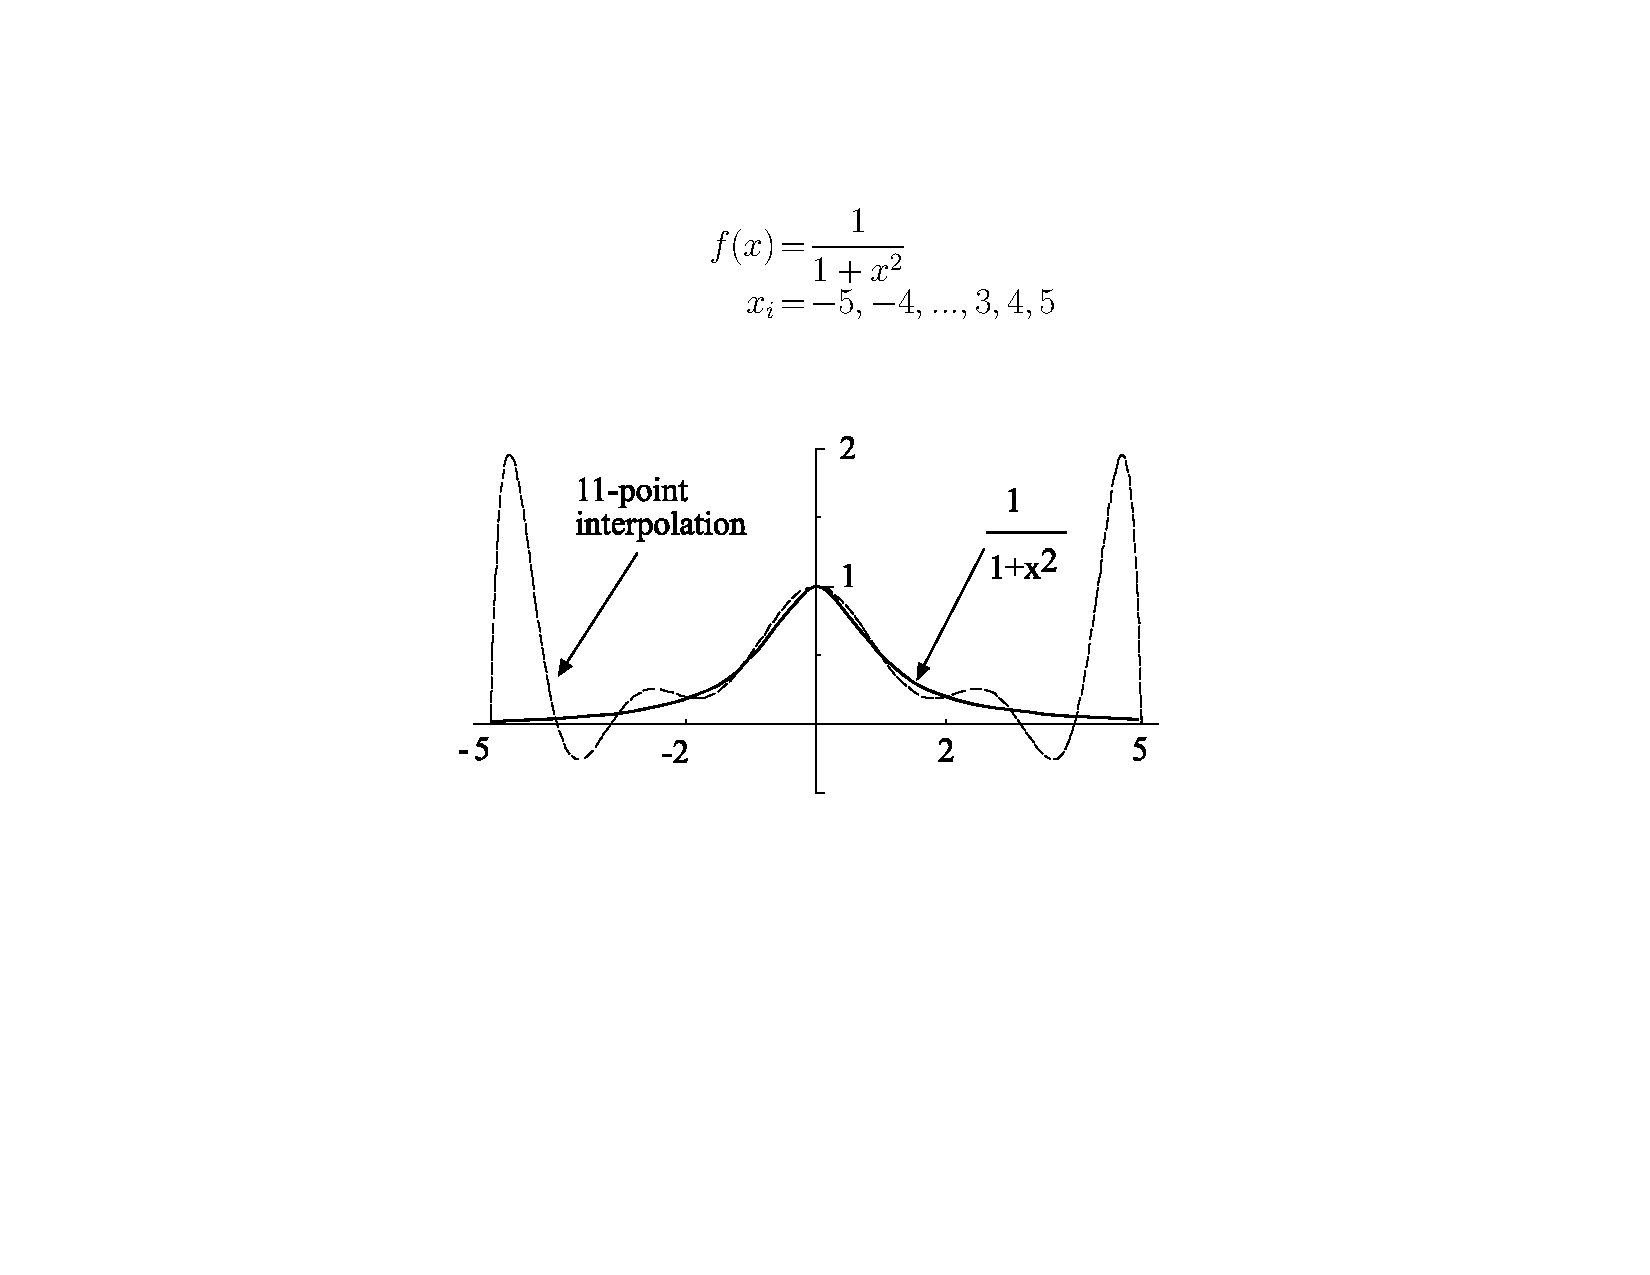
\includegraphics[height=2.8in]{./resources/functionalapprox.pdf}
\end{center}
\end{figure}
\end{frame}

\begin{frame}{Interpolation Methods  (Judd Ch 6)}
\begin{block}{Hermite Polynomial Interpolation}
\begin{itemize}
\item Data $(x_i,y_i,y'_i)$, $i=1,\ldots,n$
\item Objective, find an $2n-1$ degree polynomial $p_n(x)$ which agrees with the data $y_i = p(x_i)$ AND $y'_i = p'(x_i)$
\item Result: If $x_i$ are distinct there is a unique interpolating polynomial
\end{itemize}
\end{block}
\begin{block}{Least Squares Approx}
\begin{itemize}
\item Data the function $f(x)$
\item Objective: find a function $g(x)$ in class $G$ that best approximates $f(x)$ ie:
\begin{eqnarray*}
g = \arg \min_{g \in G} \| f-g\|^2
\end{eqnarray*}
\end{itemize}
\end{block}
\end{frame}

\begin{frame}{Orthogonal Polynomials}
\begin{block}{General Case}
\begin{itemize}
\item Space: polynomials over domain $D$
\item Weighting function: $w(x) > $ (positive everywhere)
\item Inner product $\langle f,g \rangle = \int_D f(x) g(x) w(x) d x$
\item Polynomials are orthogonal wrt to $w(x)$ IFF 
\begin{eqnarray*}
\langle \phi_i, \phi_j \rangle = 0, \quad i \neq j
\end{eqnarray*}
\item Can compute orthogonal polynomials using recurrence formulas
\begin{eqnarray*}
\phi_0(x) &=& 1\\
\phi_1(x) &=& x \\
\phi_{k+1}(x) &=& (a_{k+1} x + b_k) \phi_k(x) + c_{k+1} \phi_{k-1}(x)
\end{eqnarray*}
\end{itemize}
\end{block}
\end{frame}

\begin{frame}{Chebyshev Polynomials}
\begin{itemize}
\item Can compute orthogonal polynomials using recurrence formulas
\item $[a,b] = [-1,1]$ and $w(x) = (1-x^2)^{-1/2}$
\item $T_n(x) = \cos(n \cos^{-1} x)$
\item Recursive Definition 
\begin{eqnarray*}
T_0(x) &=& 1\\
T_1(x) &=& x\\
T_{n+1}(x) &=& 2x T_n(x) - T_{n-1}(x)
\end{eqnarray*}
\end{itemize}
\begin{block}{General Intervals}
\begin{itemize}
\item Most problems aren't on the $[-1,1]$ interval so we need a COV
\begin{eqnarray*}
y = -1 + 2 \frac{x-a}{b-a}
\end{eqnarray*}
\item Polynomials $\phi_i^{*}(x) \equiv \phi_i (-1 + 2 \frac{x-a}{b-a})$ are orthogonal over $x \in[a,b]$ with respect to the weight $w^{*}(x) \equiv (-1 + 2 \frac{x-a}{b-a})$ iff the $\phi_i(y)$ are orthogonal over $y\in[-1,1]$ wrt $w(y)$.
\end{itemize} 
\end{block}
\end{frame}

\begin{frame}{Chebyshev Approximation Algorithm}
\begin{enumerate}
\item Compute the $m \geq n+1$ Chebyshev nodes on $[-1,1]$
\begin{eqnarray*}
z_k = -\cos \left ( \frac{2k-1}{2m} \pi \right) , \quad k=1,\ldots,m
\end{eqnarray*}
\item Adjust the nodes to $[a,b]$ interval
\begin{eqnarray*}
x_k = (z_k + 1)\left(\frac{b-a}{2} \right) + a , \quad k=1,\ldots,m
\end{eqnarray*}
\item Evaluate $f$ at the nodes $w_k = f(x_k)$ for $ k=1,\ldots,m$
\item Compute the coefficients $a_i$ to get the approximation $p(x)$
\begin{eqnarray*}
a_i &=& \frac{\sum_{k=1}^m w_k T_i(z_k)}{\sum_{k=1}^m  T_i(z_k)^2} \\
p(x) &=& \sum_{i=0}^n a_i T_i \left( 2 \frac{x-a}{b-a} -1 \right) 
\end{eqnarray*}
\end{enumerate}
\end{frame}

\begin{frame}{Minimax Approximation}
\begin{itemize}
\item Data: $(x_i,y_i)$, $i=1,\ldots,n$
\item Objective: $L^{\infty}$ fit
\begin{eqnarray*}
\min_{\beta \in R^m} \max_{i} \| y_i - f(x_i; \beta) \|
\end{eqnarray*}
\item Difficult to do (minimax problems are non-convex)
\item Chebyshev Approximation satisfies this property, for $C^2,C^3$ functions but doesn't get $f'(x)$ right!
\end{itemize}
\begin{theorem}
Suppose $f: [-1,1] \rightarrow R$ is $C^k$ for some $k \geq 1$, and let $I_n$ be the degree $n$ polynomial interpolation of $f$ based at the zeroes of $T_{n+1}(x)$ then
\begin{eqnarray*}
\tiny
\| f - I_n \|_{\infty} \leq \left(\frac{2}{\pi}  \log(n+1) + 1 \right) \frac{(n-k)!}{n!} \left ( \frac{\pi}{2}\right)^k  \left ( \frac{b-a}{2}\right)^k \| f^{(k)} \|_{\infty}
\end{eqnarray*}
\end{theorem}
\end{frame}


\begin{frame}{Splines}
Splines are piecewise interpolating functions
\begin{definition} 
A function $s(x)$ on $[a,b]$ is a spline of order $n$ IFF
\begin{enumerate}
\item $s$ is $C^{n-2}$ on $[a,b]$ and 
\item there is a grid of points (nodes) $a = x_0 < x_1 < \cdots < x_m = b$ such that $s(x)$ is a polynomial of degree $n-1$ on each subinterval $[x_i, x_{i+1}]$, $i = 0,\ldots,m-1$
\end{enumerate}
\end{definition}
Second order plane is piecewise linear.\\
We usually use cubic splines.
\end{frame}


\begin{frame}{Splines}
Cubic Splines
\begin{itemize}
\item Lagrange data set $(x_i,y_i)$ for $i=0,\ldots n$.
\item Nodes: the $x_i$ are the nodes of the spline
\item Functional form $s(x) = a_i + b_i x + c_i x^2 + d_i x^3$ on $[x_{i-1},x_i]$
\item Unknowns $4n$ unknown coefficients
\item $2n$ interpolation and continuity conditions:
\begin{eqnarray*}
y_i &=& a_i + b_i x_i + c_i x_i^2 + d_i x_i^3 \quad i=1,\dots, n\\
y_i &=& a_{i+1} + b_{i+1} x_i + c_{i+1} x_i^2 + d_{i+1} x_i^3 \quad i=0,\ldots, n-1
\end{eqnarray*}
\item $2n - 2$ conditions from $C^2$ at the interior for $i=1,\ldots,n-1$
\begin{eqnarray*}
b_i + 2c_i x_i + 3 d_i x_i^2  &=& b_{i+1} + 2 c_{i+1} x_i + 3 d_{i+1}x_i^2\\ 
2c_i + 6d_i x_i &=& 2c_{i+1} + 6d_{i+1} x_i
\end{eqnarray*}
\end{itemize}
\end{frame}


\begin{frame}{Side Conditions}
We have $4n-2$ linear equations and $4n$ unknowns we need two side conditions to identify the system
\begin{itemize}
\item Natural spline: $s''(x_0) = s''(x_n) = 0$ minimizes the total curvature $\int_{x_0}^{x_n} s''(x)^2 dx$
\item Hermite spline: $s'(x_0) = y_0'$ and $s'(x_n) = y_n'$ (with extra data)
\item Secant Hermite: $s'(x_0) = \frac{s(x_1) - s(x_0)}{x_1-x_0}$ , $s'(x_n) = \frac{s(x_n) - s(x_{n-1})}{x_n-x_{n-1}}$
\item Solvers are built in to packages like MATLAB (check documentation for which method).
\end{itemize}
\end{frame}


\begin{frame}{Shape Issues}
\begin{figure}[htbp]
\begin{center}
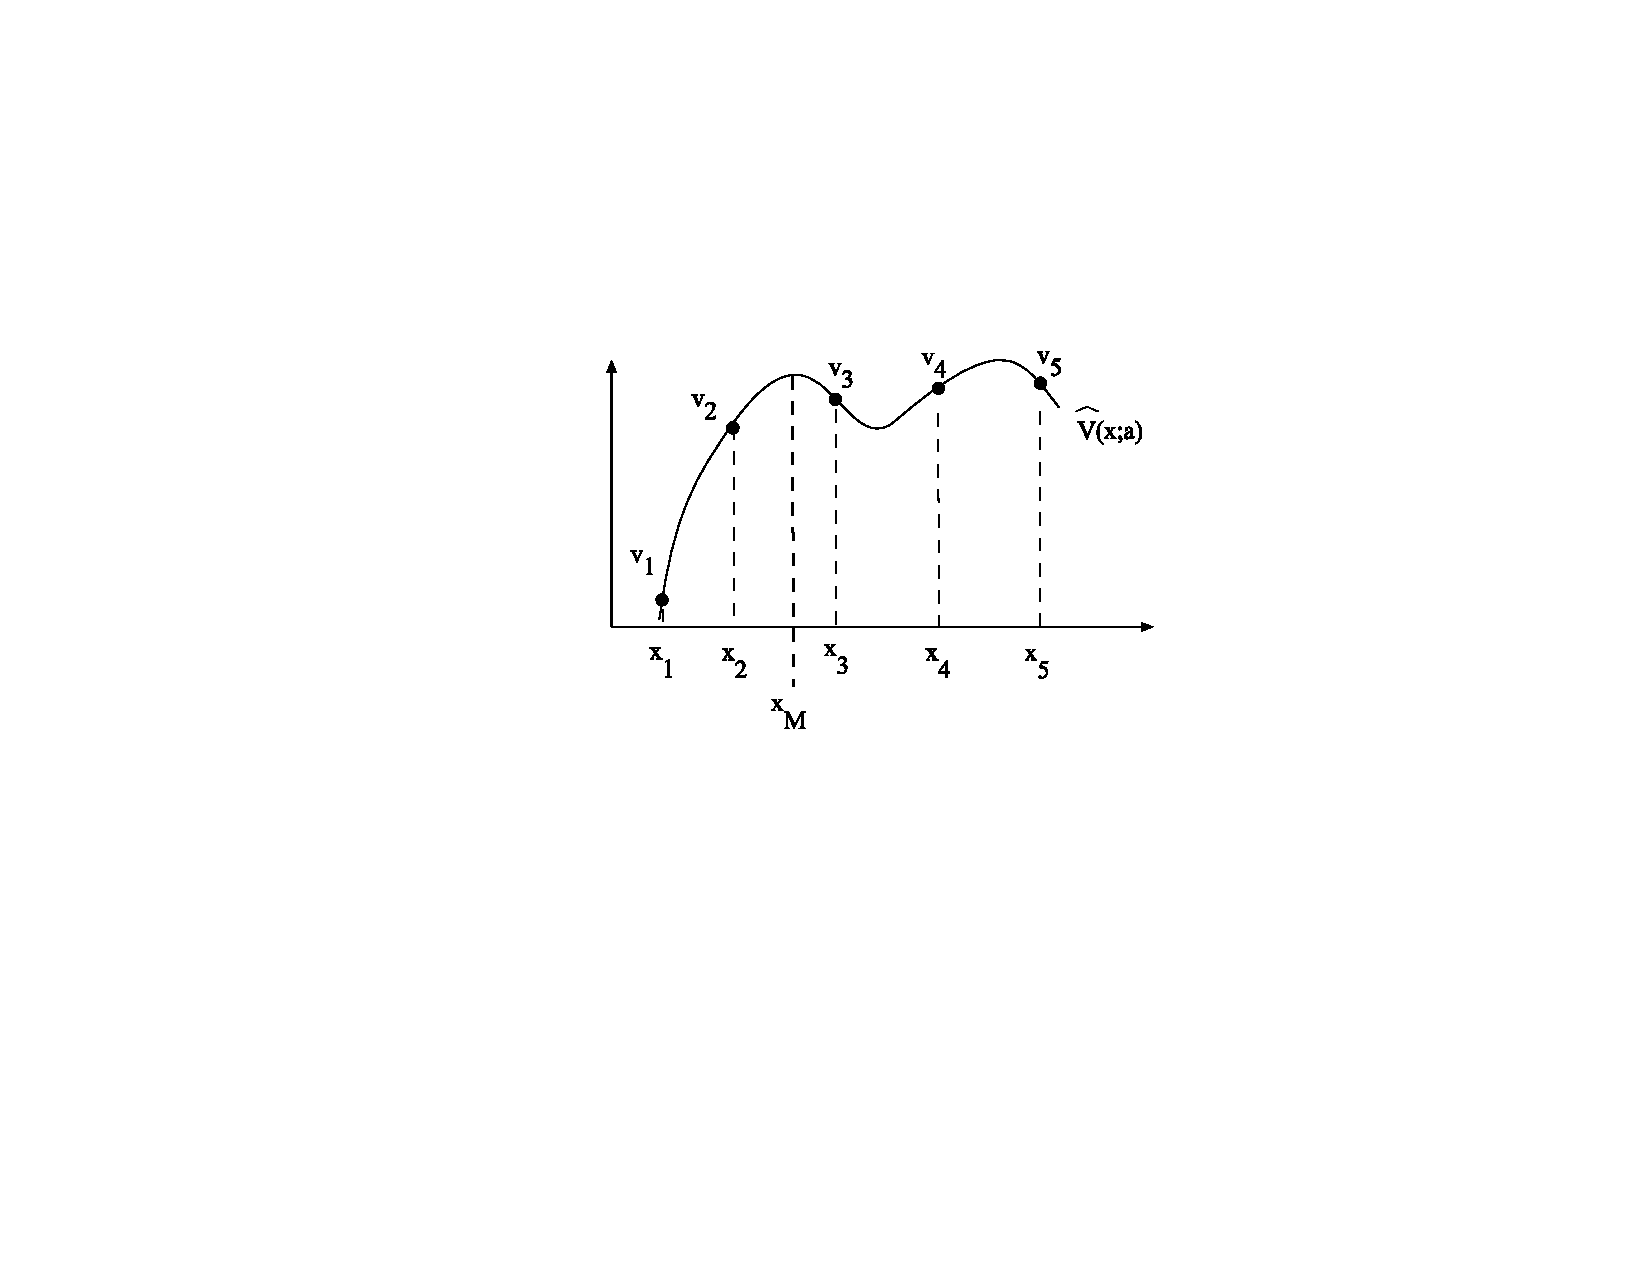
\includegraphics[height=2in]{./resources/spline.pdf}
\label{default}
\end{center}
\end{figure}
\begin{itemize}
\item Concave (monotone) data may lead to non concave (non monotone) approximations
\item Shape problems stabilize VFI.
\end{itemize}
\end{frame}

\begin{frame}{Schumaker Procedure (Shape Preserving Splines)}
\begin{enumerate}
\item Take level (and maybe slope) data at nodes $x_i$
\item Add intermediate nodes $z_i^{+} \in [x_i,x_{i+1}]$
\item Run quadratic spline with nodes at the $x$ and $z$ nodes which interpolate data and preserves shape
\item Schumaker formulas tell you how to choose the $z$ and spline coefficient
\item Detail in Judd and in companion paper (Judd and Solnick)
\end{enumerate}
\end{frame}


\begin{frame}{Numerical Integration}
We are interested in lots of problems that require computing difficult integrals (e.g.: evaluating expectations )
\begin{enumerate}
\item Midpoint/Trapezoid Rules
\item Simpson's Rule
\item Gaussian Rules
\item Higher-Dimensional Rules
\end{enumerate}
\end{frame}


\begin{frame}{Quadrature Rules}
Basic idea of quadrature is to approximate complicated functions with something easier to integrate, and then integrate that exactly.\\
\begin{figure}[htbp]
\begin{center}
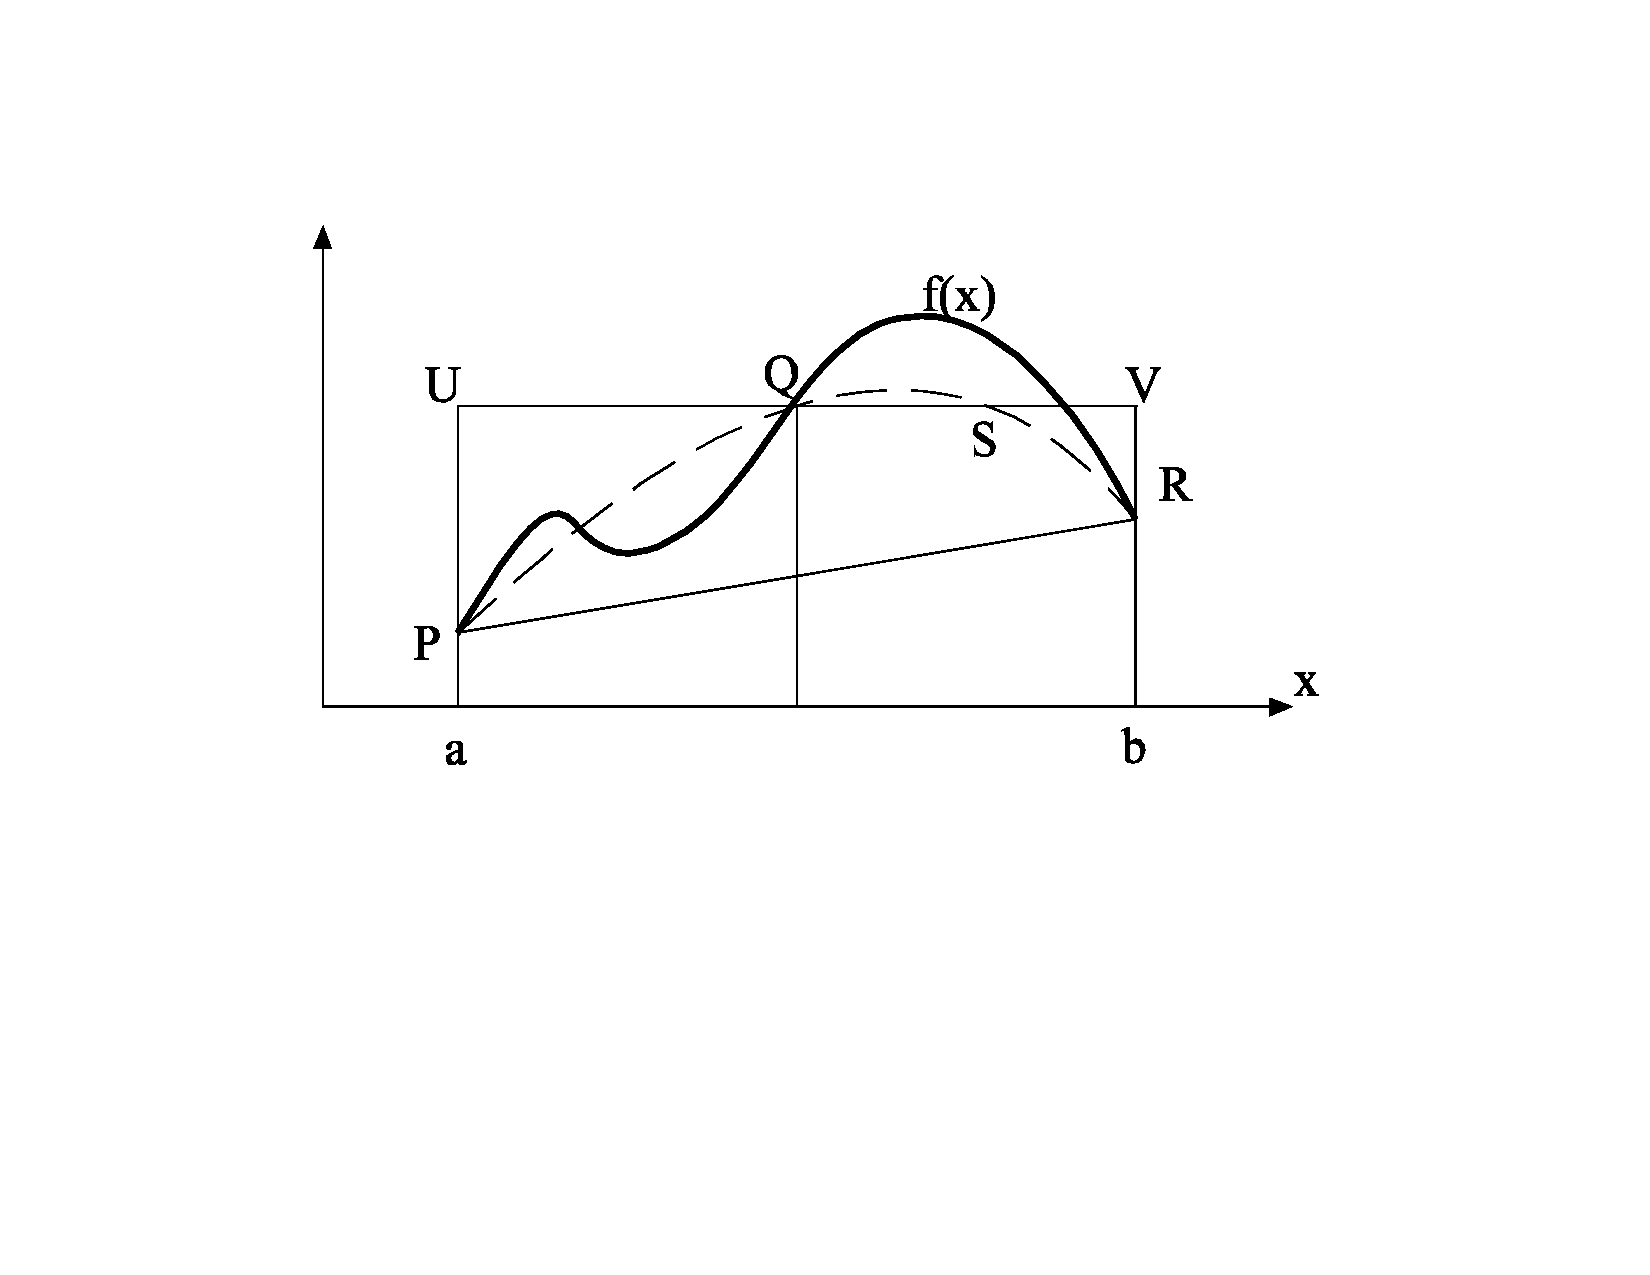
\includegraphics[height=1.75in]{./resources/quadrature.pdf}
\end{center}
\end{figure}
\begin{itemize}
\item Constant $f(x)$ at midpoint of $[a,b]$ $aUQVb$ for box.
\item Linear: Trapezoid $a PRb$
\item Parabola through $f(x)$ at $a,b$ and $\frac{a+b}{2}$ for $aPQRb$
\end{itemize}
\end{frame}

\begin{frame}{Simpsons Rule (Newton-Cotes)}
Piecewise Quadratic Approximation at some $\xi \in[a,b]$
\begin{eqnarray*}
\int_{a}^b f(x) d x \approx \left(\frac{b-a}{6} \right) \left[f(a) + 4f \left( \frac{a+b}{2} \right) + f(b) \right]  - \frac{(b-a)^5}{2880} f^{(4)} (\xi)
\end{eqnarray*}
With approximation error
\begin{eqnarray*}
\frac{1}{90} \left( \frac{b-a}{2}\right)^5 | f^{(4)} (\xi) |
\end{eqnarray*}
Works well when quadratic approximation is good $f^{(4)}$ is small or interval is small.
\end{frame}

\begin{frame}{Gaussian Quadrature}
Formulas of the form
\begin{eqnarray*}
\int_{a}^b f(x) d x \approx \sum_{i=1}^n  w_i f(x_i)
\end{eqnarray*}
for some quadrature nodes $x_i \in [a,b]$ and weights $w_i$.
\begin{itemize}
\item Let $\mathcal{F}_k$ be the space of degree $k$ polynomials
\item Quadrature formulas are exact of degree $k$ if it correctly integrates each function in $\mathcal{F}_k$
\item Gaussian quadrature formulas use $n$ points and are exact of degree $2n-1$.
\end{itemize}
Approximation Error
\begin{eqnarray*}
(f,g) = \int_a^b w(x) f(x)  dx - \sum_{i=1}^n w_i f(x_i) = \frac{f^{(2n)}(\xi)}{(2n)!} (p_n,p_n) 
\end{eqnarray*}
\end{frame}

\begin{frame}{Gaussian Quadrature}
\begin{description}
\item[Legendre] Domain: $[-1,1]$, $w(x) = 1$
\item[Chebyshev] Domain: $[-1,1]$, $w(x) = \frac{1}{\sqrt{1-x^2}}$
\item[Laguerre] Domain: $[0,\infty]$, $w(x) = \exp[-x]$ (useful for present value)
\item[Hermite] Domain: $[-\infty,\infty]$, $w(x) = \exp[-x^2]$ (useful for normal)
\end{description}
Helpful if function is $C^{\infty}$ or analytic.
\end{frame}

\begin{frame}{Gauss Herrmite}
Let $Y\sim N(\mu,\sigma^2)$ and apply COV $x = (y-\mu)/\sqrt{2} \sigma$
\begin{eqnarray*}
E[f(Y)] = (2 \pi \sigma^2)^{-\frac{1}{2}} \int_{-\infty}^{\infty} f(y) \exp\left[-\frac{(y-\mu)^2}{2\sigma^2} \right] dy \\
\int_{-\infty}^{\infty} f(y) \exp\left[-\frac{(y-\mu)^2}{2\sigma^2} \right] dy = \int_{-\infty}^{\infty} f(\sqrt{2} \sigma x + \mu) e^{-x^2} \sqrt{2} \sigma dx
\end{eqnarray*}
Gives the quadrature formula using Gauss Hermite $(x_i,w_i)$.
\begin{eqnarray*}
E[f(Y)] = \frac{1}{\sqrt{\pi}} \sum_{i=1}^n w_i f(\sqrt{2}\sigma x_i + \mu)
\end{eqnarray*}
\end{frame}

\begin{frame}{Higher Dimensional Integration}
\begin{itemize}
\item In higher dimension we can use product rules of 1-D integrals.
\item This grows exponentially in dimension $D$ (Curse of Dimensionality)
\item Monte Carlo is not cused but slow to converge $\frac{1}{\sqrt{n}}$ vs $\frac{1}{2n!} f^{(2n)}$
\item Some monomial rules (Judd), (Skrainka and Judd) aren't cursed
\item Sparse Grids show how to combine 1-D rules more efficiently (www.sparse-grids.de)
\end{itemize}
\end{frame}



\end{document}